\subsection{Aufbau des Prototypen}\label{hw_prototype}
Der Prototyp war eine Kombination aus dem verwendeten Touchscreen sowie dem Raspberry Pi 4 und dem Zigbee-Stick. 
Dieser Prototyp diente als Entwicklungsplattform für die Software.
\begin{figure}[H]
	\begin{subfigure}[b]{0.5\linewidth}
		\includegraphics[width=1\textwidth]{img/prototype_front.png}
		\caption[Vorderseite des Prototypen]{Vorderseite des Prototypen}
	\end{subfigure}
	\begin{subfigure}[b]{0.5\linewidth}
		\includegraphics[width=1\textwidth]{img/prototype_back.png}
		\caption[Rückseiteseite des Prototypen]{Rückseite des Prototypen}
	\end{subfigure}
	\begin{subfigure}[b]{1\linewidth}
		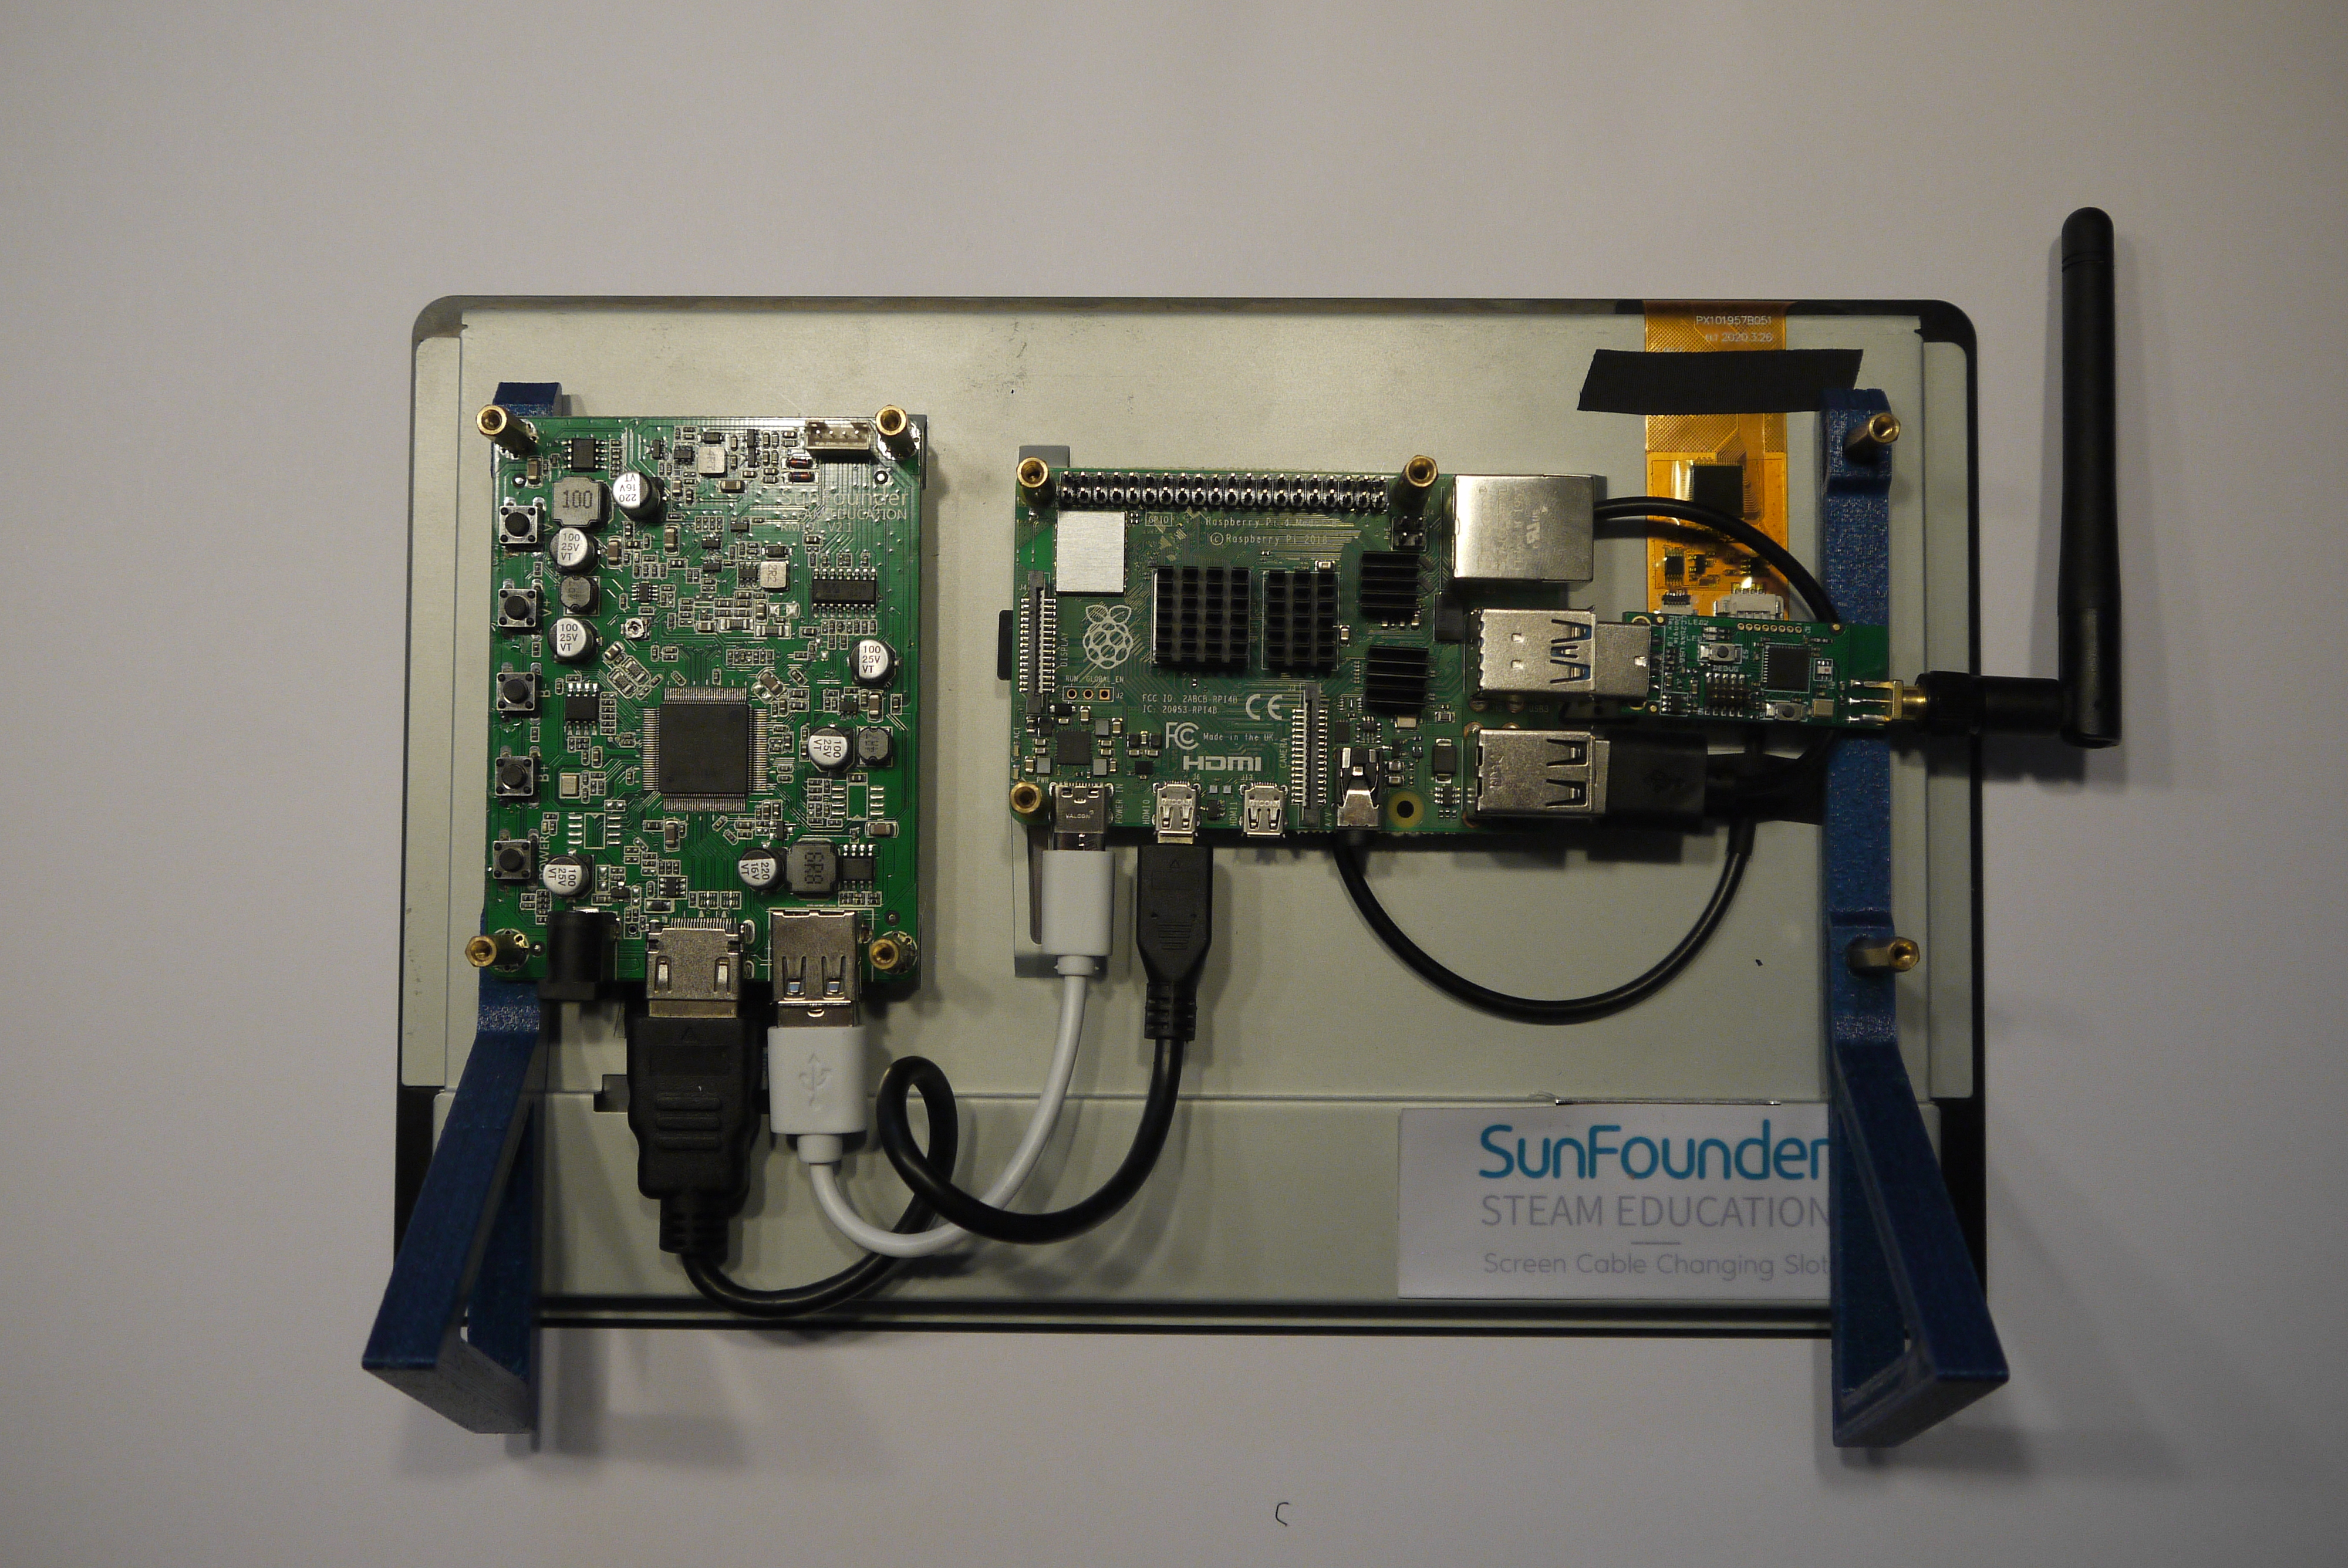
\includegraphics[width=1\textwidth]{img/prototype_back_detail.png}
		\caption[Detailansicht der Rückseite]{Detailansicht der Rückseite}
	\end{subfigure}
	\caption[Prototyp der Smart Home Zentrale]{Prototyp der Smart Home Zentrale}
	\label{prototype}
\end{figure}
\newpage